
\chapter{C++ Implementation}




\section{Introducing High Level Target Language}

We can get a high level view of the changes a compiler makes.
We can abstract compilation features we are not interested in
and concentrating the featues we are interested in. 
For us, we are interested in reasoning about high level features. 
We are not interested in details such as 
memory alignment, types, sizes, machine code instructions.
In fact, we abstract away enough so our view will be independent of 
any machine's instruction set.

\begin{itemize}   
\renewcommand{\labelitemi}{$\Box$}
\item \textbf{Identifiers} The set $Ident$ is a set of identifiers $x$. 
\item \textbf{Memory} A given memory $m$ is a map $m : Int \rightarrow Int \cup Ident$ to the set. 
We assume a word addressed machine. $m(x)$ addresses word number $x$. 
We assume that identifier addresses take up \textit{one word}. 
There is a \textit{position function} $\pi : Ident \rightarrow int$ gives a memory for each identifier.
\end{itemize} 

The syntax of the C++ HLTL is shown below.

$$Loc ::= IntConst \;|\; \alpha(Ident) \;|\; \star Loc \;|\; Loc + Loc $$


Now we describe the operation semantics for $Loc$.
We define a location evaluation $\leadsto_L$. 

\highlightdef{\textbf{Location Evaluation}: 
$\leadsto_L : Int \times (Ident \rightarrow Int) 
\times (Int \rightarrow Int \cup Ident) \rightarrow Int$ }


\begin{prooftree}
\def\defaultHypSeparation{\hskip .01in}
\AxiomC{}
\LeftLabel{\textsc{const}}
\UnaryInfC{$(i, \pi, m) \leadsto_L i$}
\end{prooftree}

This first axiom states that a constant integer representing 
the address of word in memory evaluates to that very constant integer. 

\begin{prooftree}
\def\defaultHypSeparation{\hskip .01in}
\AxiomC{}
\LeftLabel{\textsc{pos}}
\UnaryInfC{$(\alpha(x), \pi, m) \leadsto_L \pi(i)$}
\end{prooftree}

The next axiom is for the identifier \textit{position operator} $\alpha$. The rule says that 
the deferencing operator gives the location of an identifer, 
which is given by the \textit{position function} $\pi$. 
Note that the difference between $\alpha$ and $\pi$ is that 
$\alpha$ is part of the syntax of the high level target language - 
whereas $\pi$ is not. We use $\pi$ to, describe the operational semantics
of $\alpha$, and to describe other semantics. 

\begin{prooftree}
\def\defaultHypSeparation{\hskip .01in}
\AxiomC{$(loc, \pi, m) \leadsto_L i$}
\LeftLabel{\textsc{deref}}
\UnaryInfC{$(\star loc, \pi, m) \leadsto_L m(i)$}
\end{prooftree}

The next rule is for the deferencing operator $\star$. Given any location 
$loc$, we use $\star$ to see the \textit{contents} of the memory address 
that $loc$ refers to. If $loc$ location-evaluated to $i$, then the location 
$loc$ refers to is $i$ and so the memory contents are given by $m(i)$.  
So overall, $\star loc$ location-evaluates to $m(i)$. 

\begin{prooftree}
\def\defaultHypSeparation{\hskip .01in}
\AxiomC{$(loc, \pi, m) \leadsto_L i$}
\AxiomC{$(loc', \pi, m) \leadsto_L i'$}
\LeftLabel{\textsc{add}}
\BinaryInfC{$(loc + loc', \pi, m) \leadsto_L i + i'$}
\end{prooftree}

The next rule allows us to add two addresses together. 
We define the semantics for $Loc + Loc$. Suppose we 
have two locations $loc,loc' \in Loc$.  
Intuitively, if location $loc$ evaluates to integer $i$ and 
another location $loc'$ evaluates to integer $i'$ then 
$loc + loc'$ evaluates to integer $i + i'$. 

\frmrule

\begin{example}



\end{example}

\frmrule  

We now add instructions to HLTL. 
Instructions allow us to modify the contents of memory. Below shows the syntax 
for instructions $Instr$ and method bodies $MethBody$.

$$Instr ::= Instr;Instr \;|\; Loc := Loc \;|\; Ident(Loc^{*}) \;|\; Loc(Loc^{*}) $$
$$MethBody ::= Ident^{*} \{ Instr^{*} \}$$

Now we describe the operation semantics for instructions by
defining an instruction evaluation $\leadsto_I$. 

\highlightdef{\textbf{Instruction Evaluation}: 
$\leadsto_I : Instr \times (Ident \rightarrow Int) \times (Int \rightarrow Int \cup Ident)
\rightarrow (Int \rightarrow Int \cup Ident)$ }


\begin{prooftree}
\def\defaultHypSeparation{\hskip .01in}
\AxiomC{$(loc := loc', \pi, m) \leadsto_I i$}
\AxiomC{$(loc := loc', \pi, m) \leadsto_I i'$}
\LeftLabel{\textsc{assign}}
\BinaryInfC{$(loc := loc', \pi, m) \leadsto_I m[i \mapsto i']$}
\end{prooftree}

This rule updates the memory to reflect an assignment. 
The location indicated by $loc$ is updated to the location indiciated 
by $loc'$. If $loc'$ location-evaluates to $i'$ then this is what should 
be in whatever location $loc'$ location-evaluates to, $i$. 
Hence the instruction updates the memory function $m$ to $m[i \mapsto i']$ 
where all mappings are unchanged except that now $i$ maps to $i'$. 

\begin{prooftree}
\def\defaultHypSeparation{\hskip .01in}
\AxiomC{$(instrs, \pi, m) \leadsto_I m'$}
\AxiomC{$(instr, \pi, m') \leadsto_I m''$}
\LeftLabel{\textsc{seq}}
\BinaryInfC{$(instrs;instr, \pi, m) \leadsto_I m''$}
\end{prooftree}

The next rule is for creating sequences of instructions. 
The rule tells us that the evaluation of $instrs;instr$ 
requires that we instruction-evaluate $instrs$, then take the 
memory contents of that evaluation and 
use them to instruction-evaluate $instr$ to give the final memory 
contents.



\begin{prooftree}
\def\defaultHypSeparation{\hskip .01in}
\AxiomC{
$
\begin{matrix}
&
\kappa(id) = par_1 \cdots par_n \{ instrs \}
&
\\
\begin{matrix}
(loc_1, \pi, m) \leadsto_L i_1  \\
(loc_2, \pi, m) \leadsto_L i_2  \\
\cdots \\
(loc_n, \pi, m) \leadsto_L i_n \\
(instrs, \pi', m') \leadsto_I m'' \\
\end{matrix}
&
\pi' =
\begin{matrix}
par_1 \mapsto i_1'  \\
par_2 \mapsto i_2'  \\
\cdots \\
par_n \mapsto i_n'
\end{matrix}
&
m' = m\left[
\begin{matrix}
i_1' \mapsto i_1  \\
i_2' \mapsto i_2  \\
\cdots \\
i_n' \mapsto i_n
\end{matrix}\right]
\end{matrix}
$
}
\LeftLabel{\textsc{func}}
\UnaryInfC{$(id(loc_1, \cdots, loc_n), \pi, m) \leadsto_I m''$}
\end{prooftree}


When we call a method, the idea is to create a new lexical scope, $pi'$, similar 
to how function calls have their own scope. 
This scope will bind the parameters identifiers $par_1 \cdots, par_n$
to our argument identifiers $loc_1 \cdots, loc_n$. 

Suppose that the arguments $loc_1 \cdots, loc_n$ location-evaluate to $i_1, \cdots i_n$ , 
then it is these memory locations that hold the argument values. 
In essence, $i_1, \cdots i_n$ are integer constants that are 
\textit{references} to the argument values. 
Performing $\star i_k$ gives the $k$th argument's value. 



\begin{tikzpicture}
  %
  \tikzstyle{m} = [draw=black!50, minimum width=1.5cm, minimum height=0.5cm, inner sep = 0.2pt, font=\small]
  \tikzstyle{m2} = [m, fill=black!5, draw=black!50]
  \matrix[row sep=-0.01cm, column sep=-0.01cm] (memory) 
  {
    \node[m]{}; & \node[m]{}; \\
    \node[m]{}; & \node[m]{}; \\
    \node[m]{}; & \node[m]{}; \\
    \node[m]{}; & \node[m]{}; \\
    \node[m2](i1){$i_1'$}; & \node[m2]{$i_1$}; \\
    \node[m2](i2){$i_2'$}; & \node[m2]{$i_2$}; \\
    \node[m2](ietc){$\cdots$}; & \node[m2]{$\cdots$}; \\
    \node[m2](in){$i_n'$}; & \node[m2]{$i_n$}; \\
  };
  \node[left=1.4cm of i1](par1){$par_1$}; 
  \node[left=1.4cm of i2](par2){$par_2$}; 
  \node[left=1.4cm of ietc](paretc){$\cdots$}; 
  \node[left=1.4cm of in](parn){$par_n$}; 
  \draw[|->,>=stealth',shorten >=3pt] (par1) -- (i1);
  \draw[|->,>=stealth',shorten >=3pt] (par2) -- (i2);
  \draw[|->,>=stealth',shorten >=3pt] (paretc) -- (ietc);
  \draw[|->,>=stealth',shorten >=3pt] (parn) -- (in);
  \node at ($(par1)+(1.0cm,0.5cm)$) {$\pi'$};
  \draw[decorate,decoration={brace},thick]
      ($(memory.north west)+(0.1cm,0.1cm)$) to node[midway,above,yshift=0.1cm] {$m'$}
      ($(memory.north east)+(-0.1cm,0.1cm)$);
\end{tikzpicture}



% Add Prooftree


Now we need to decide whether to \textit{pass by value} or we \textit{pass by reference}.
We have decided to write the operational semenatics such that every parameter for 
every method call uses \textit{pass by value}. We need to work out how to 
create references to our parameter values. 

Notice that if we did \textit{pass by reference}, then our parameters would location-evaluate to 
$i_1, \cdots i_n$, just as how location-evaluating the arguments themselves gives 
$i_1, \cdots i_n$. Our parameters would simply be aliases.
However we are adopting \textit{pass by value}. We don't want our 
parameters to evaluate directly to the memory addresses of the values. 
We need to add a level of indirection.
Instead, our parameters should location-evaluate to some new address $i_1', \cdots i_n'$ whose 
memory contents contain the direct memory addresses $i_1, \cdots i_n$ to the argument values. 

So to add this level of indirection, we add to memory $m$ new mappings, 
$m' = m[i_1' \mapsto i_1, i_2' \mapsto i_2, \cdots, i_n' \mapsto i_n]$, 
to create new addresses $i_1', \cdots i_n'$ whose 
memory contents contain the reference $i_1, \cdots i_n$ to the argument values. 
Now we just need to direct our parameters to $i_1', \cdots, i_n'$.

We create a new scope by creating a new $\pi'$ with 
just the mappings $par_1 \mapsto i_1'$, $par_2 \mapsto i_2'$, ..., $par_n \mapsto i_n'$
This allows our parameters to location-evaluate to the new address $i_1', \cdots, i_n'$. 


\begin{prooftree}
\def\defaultHypSeparation{\hskip .01in}
\AxiomC{
$
\begin{matrix}
(loc, \pi, m) \leadsto_L i \\
m(i) = id \\
(id(loc_1, \cdots, loc_n), \pi, m) \leadsto_I m'
\end{matrix}
$
}
\LeftLabel{\textsc{funcpoint}}
\UnaryInfC{$(loc(loc_1, \cdots, loc_n), \pi, m) \leadsto_I m'$}
\end{prooftree}


The next rule allows us to have \textit{function pointers}.
The previous rule only allows us to call functions using 
identifiers that are defined in $\kappa$. 
Rather than having just function calls via \textit{identifiers}, 
we could also have function calls via \textit{locations}.

If the memory contents given by some location $loc$ has a identifier $id$
and we know that a function call with that identifier is valid (it 
instruction evaluates to some memory) - 
then performing the function call \textit{using the location} 
makes sense. 

In essence, $loc$ acts as a function pointer. We are adding a level of 
indirection for calling functions. We can roughly think of 
$loc$ are pointing to a function $id$ that's defined in $\kappa$.
We can change the function that $loc$ points to by changing $m(i)$
from $id$ to some new $id'$ that's also has a mapping defined in $\kappa$. 


\frmrule

\begin{example}
Assume that $\pi(x) = 300, \pi(y) = 400$ for identifiers $x,y \in Ident$. \\
For the initial memory contents shown below, show the resulting memory 
after the execution of the following instructions.

$$\alpha(x) + 1 := \alpha(y); \;\;\;
\alpha(x)+2 := \star(\alpha(x)+1); \;\;\;
\alpha(x+3) := \star(\alpha(x))+1;$$

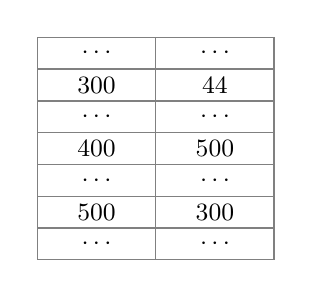
\begin{tikzpicture}
  %
  \tikzstyle{m} = [draw=black!50, minimum width=1.5cm, minimum height=0.4cm, inner sep=0.1pt, font=\small]
  \matrix[row sep=-0.01cm, column sep=-0.01cm] (memory) 
  {
    \node[m]{$\cdots$}; & \node[m]{$\cdots$}; \\
    \node[m]{300}; & \node[m]{44}; \\
    \node[m]{$\cdots$}; & \node[m]{$\cdots$}; \\
    \node[m]{400}; & \node[m]{500}; \\
    \node[m]{$\cdots$}; & \node[m]{$\cdots$}; \\
    \node[m]{500}; & \node[m]{300}; \\
    \node[m]{$\cdots$}; & \node[m]{$\cdots$}; \\
  };
\end{tikzpicture}
\end{example}

\frmrule

\begin{example}
Assume that $\pi(x) = 300, \pi(y) = 400$ for identifiers $x,y \in Ident$. \\
For the initial memory contents shown below, show the resulting memory 
after the execution of the following instructions.

$$
\star(\star(\alpha(y))) := 10; \;\;\;
\star(\alpha(x)) := 100; \;\;\;
\alpha(y) := 1000;
$$

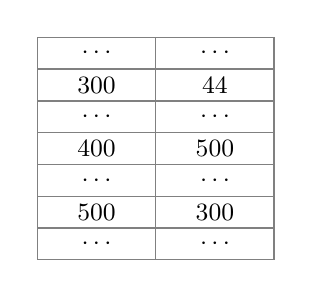
\begin{tikzpicture}
  %
  \tikzstyle{m} = [draw=black!50, minimum width=1.5cm, minimum height=0.4cm, inner sep=0.1pt, font=\small]
  \matrix[row sep=-0.01cm, column sep=-0.01cm] (memory) 
  {
    \node[m]{$\cdots$}; & \node[m]{$\cdots$}; \\
    \node[m]{300}; & \node[m]{44}; \\
    \node[m]{$\cdots$}; & \node[m]{$\cdots$}; \\
    \node[m]{400}; & \node[m]{500}; \\
    \node[m]{$\cdots$}; & \node[m]{$\cdots$}; \\
    \node[m]{500}; & \node[m]{300}; \\
    \node[m]{$\cdots$}; & \node[m]{$\cdots$}; \\
  };
\end{tikzpicture}
\end{example}

\frmrule

\begin{example}
Assume $\kappa(f) = x,y \{ \star \alpha(y) := \star \star \alpha(x) \}$. \\
For the initial memory contents shown below, show the resulting memory \\
\textbf{(a)} On entry to function $f$ for some $m, \pi'$ \\
\textbf{(b)} Just before leaving function $f$ for $m', \pi'$ \\
\textbf{(c)} After execution of the function $f$ for $m'', \pi$ \\

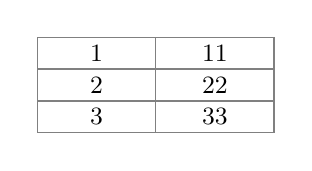
\begin{tikzpicture}
  %
  \tikzstyle{m} = [draw=black!50, minimum width=1.5cm, minimum height=0.4cm, inner sep=0.1pt, font=\small]
  \matrix[row sep=-0.01cm, column sep=-0.01cm] (memory) 
  {
    \node[m]{1}; & \node[m]{11}; \\
    \node[m]{2}; & \node[m]{22}; \\
    \node[m]{3}; & \node[m]{33}; \\
  };
\end{tikzpicture}
\end{example}

\frmrule





\section{HLTL I: Single Inheritance}

We now extend the HLTL to suppose classes and objects.  

\begin{itemize}   
\renewcommand{\labelitemi}{$\Box$}
\item \textbf{Object Layout} Lay out all fields of a class next to each 
other in memory. For each field we associated some offset $k$ where $k \geqslant 0$. 
The compiler remembers which field has what offset.  
In order to address an object, \textsf{a}, we always take the first cell, $\alpha(\textsf{a})$.
\item \textbf{Invariant for Layout}  The layout of objects of any class is 
a prefix of the layout of objects of any subclass. 
The result of this is that if \textsf{f} has offset $k$ for $\textsf{a}:\textsf{A}$, 
then \textsf{f} will also have offset $k$ for any $\textsf{a}':\textsf{A}'$ where $\textsf{A}' <: \textsf{A}$.
\item \textbf{Data Access} Offsets of data members are known at compile time. 
Thus data member access can be implemented through statically known offsets. 
\lstinline{a.f} in C++ has a location evaluation equivalent to $\star(\alpha(\textsf{a})) + k$ for some known offset $k$. 
\item \textbf{Pointer Data Access} 
A pointer \textsf{ap} that points to objects of class \textsf{A} 
can point to any subclass $\textsf{A}' <: \textsf{A}$. 
We can perform data member access using pointers.
\lstinline{a->f} in C++ has a location evaluation equivalent to $\alpha(\textsf{ap}) + k$ for 
some known offset $k$ taken from layouts for class \textsf{A}.
By our invariant for layout, 
if \textsf{f} has offset $k$ for $\textsf{a}:\textsf{A}$, 
then it must have offset $k$ for any $\textsf{a}':\textsf{A}'$ where $\textsf{A}' <: \textsf{A}$.
Hence $\star(\alpha(\textsf{ap})) + k$ will always access field \textsf{f}, regardless of 
what subclass \textsf{a} points to.
\item \textbf{Object Assignment} 
Assignment of objects corresponds to copying their fields. 
For the assignment \lstinline{a=x}.
if \textsf{a.f} is a field in \textsf{a} with offset $j$, 
then $\alpha(\textsf{x}) + j := \star(\alpha(\textsf{f})) + j$. 
That is, the contents of the field are updated to the 
location evaluation equivalent of doing a C++ data access.
Notice that $\textsf{x}:\textsf{\textsf{X}}' <: \textsf{A}$, then not all 
of it's fields will be updated. Only the fields that 
are in prefix. 
\item \textbf{Pointer Assignment} 
The assignment of pointers corresponds to 
copying of addresses. The object fields are unchanged. 
The assignment \lstinline{ap=bp} is represented as:
then $\alpha(\textsf{ap}) := \star \alpha(\textsf{bp})$. 
That is, the contents at address $\pi(\textsf{ap})$ are updated 
to the contents of $\pi(\textsf{bp})$. In other words
$m' = m[\pi(\textsf{ap}) \mapsto m(\pi(\textsf{bp}))]$.

\end{itemize} 

\frmrule

\begin{example}


\end{example}

\frmrule

\begin{tikzpicture}
  \node [fill=black!5, inner sep=4pt] (class) { 
  
\begin{lstlisting}
class A { 
 public:
  int fa1, fa2;
};
class B : public A { 
 public:
  int fb1;
};
\end{lstlisting} 
  };

  \node [fill=black!5, inner sep=4pt, right=0.1cm of class] { 
\begin{lstlisting}
void main()
{
 A a1; B b1;
 a.fa1 = 3; a.fa2 = 5;
 b.fa1 = 4; a.fa2 = 6; a.fb1 = 8;

 A *ap1 = new B();
 ap->fa1 = 5; ap->fa2 = 7;
 A *bp1 = new B();
 bp->fa1 = 1; bp->fa2 = 4; bp->fb1 = 9;
};
\end{lstlisting} 
  };

\end{tikzpicture}



\begin{tikzpicture}
  %
  \tikzstyle{m} = [draw=black!50, minimum width=1.5cm, minimum height=0.4cm, inner sep=0.1pt, font=\small]
  \tikzstyle{m2} = [m, minimum width=2.2cm]
  \tikzstyle{b} = [fill=black!10]

  \matrix[row sep=-0.01cm, column sep=-0.01cm] (mema) 
  {
    \node[m]{$\cdots$}; & \node[m]{$\cdots$}; \\
    \node[m,b](fa1){$\pi(\textsf{a1})$}; & \node[m,b]{3}; \\
    \node[m,b](fa2){$\pi(\textsf{a1})$+1}; & \node[m,b]{5}; \\
    \node[m]{$\cdots$}; & \node[m]{$\cdots$}; \\
  };
  \matrix[row sep=-0.01cm, column sep=-0.01cm, above right=0.0cm and 0.1cm of mema.north east, anchor=north west] (memb) 
  {
    \node[m]{$\cdots$}; & \node[m]{$\cdots$}; \\
    \node[m,b]{$\pi(\textsf{b1})$}; & \node[m,b](fa1end){4}; \\
    \node[m,b]{$\pi(\textsf{b1})+1$}; & \node[m,b](fa2end){6}; \\
    \node[m,b](fb1){$\pi(\textsf{b1})+2$}; & \node[m,b](fb1end){8}; \\
    \node[m]{$\cdots$}; & \node[m]{$\cdots$}; \\
  };

  \matrix[row sep=-0.01cm, column sep=-0.01cm, below right=0.6cm and 0.0cm of mema.south west, anchor=north west] (memap) 
  {
    \node[m2]{$\cdots$}; & \node[m2]{$\cdots$}; \\
    \node[m2]{$\pi(\textsf{ap1})$}; & \node[m2]{$m(\pi(\textsf{ap1}))$}; \\
    \node[m2]{$\cdots$}; & \node[m2]{$\cdots$}; \\
    \node[m2,b](fa1'){$m(\pi(\textsf{ap1}))$}; & \node[m2,b]{5}; \\
    \node[m2,b](fa2'){$m(\pi(\textsf{ap1}))+1$}; & \node[m2,b]{7}; \\
    \node[m2]{$\cdots$}; & \node[m2]{$\cdots$}; \\
  };

  \matrix[row sep=-0.01cm, column sep=-0.01cm, above right=0.0cm and 0.1cm of memap.north east, anchor=north west] 
  {
    \node[m2]{$\cdots$}; & \node[m2]{$\cdots$}; \\
    \node[m2]{$\pi(\textsf{bp1})$}; & \node[m2]{$m(\pi(\textsf{bp1}))$}; \\
    \node[m2]{$\cdots$}; & \node[m2]{$\cdots$}; \\
    \node[m2,b]{$m(\pi(\textsf{bp1}))$}; & \node[m2,b](fa1end'){1}; \\
    \node[m2,b]{$m(\pi(\textsf{bp1}))+1$}; & \node[m2,b](fa2end'){4}; \\
    \node[m2,b](fb1'){$m(\pi(\textsf{bp1}))+2$}; & \node[m2,b](fb1end'){9}; \\
    \node[m2]{$\cdots$}; & \node[m2]{$\cdots$}; \\
  };
  \begin{pgfonlayer}{background} 
      \node (l1) at ($(fa1end.east)+(1.2cm,0.0cm)$) {\textsf{fa1}}; \draw[thick] (fa1) -- (l1); 
      \node (l2) at ($(fa2end.east)+(1.2cm,0.0cm)$) {\textsf{fa2}}; \draw[thick] (fa2) -- (l2); 
      \node (l3) at ($(fb1end.east)+(1.2cm,0.0cm)$) {\textsf{fb1}}; \draw[thick] (fb1) -- (l3); 

      \node (l1) at ($(fa1end'.east)+(1.2cm,0.0cm)$) {\textsf{fa1}}; \draw[thick] (fa1') -- (l1); 
      \node (l2) at ($(fa2end'.east)+(1.2cm,0.0cm)$) {\textsf{fa2}}; \draw[thick] (fa2') -- (l2); 
      \node (l3) at ($(fb1end'.east)+(1.2cm,0.0cm)$) {\textsf{fb1}}; \draw[thick] (fb1') -- (l3); 
  \end{pgfonlayer}  

\end{tikzpicture}


\frmrule


Stroustrup’s aim was to make member function calls as 
fast as normal (global) function call. 

Member functions represented by “normal” functions, 
with additional pThis parameter, representing this. 

Through name mangling distinguish between member 
functions from different classes (and also between 
overloaded functions). 

\begin{itemize}   
\renewcommand{\labelitemi}{$\Box$}
\item \textbf{Functions} A member function \lstinline{void g(int p1,...,int pn)} \{ \}
in class A is represented by $\kappa(\textsf{g\_A}) = \textsf{pThis p1} \cdots \textsf{pn}  \{ \}$
\item \textbf{Function Calls} Calls of non-virtual member functions can be resolved 
(bound) statically.
\begin{itemize} 
\item The call \lstinline{a.g();} will be represented as $\textsf{g\_A}(\alpha(\textsf{a}))$
\item The call \lstinline{ap->g();} will be represented as $\textsf{g\_A}(\star(\alpha(\textsf{ap})))$
\end{itemize} 

\end{itemize} 

\frmrule

\begin{example}
\end{example}

\section{Revision: Dynamic Binding}


%Member functions like those shown are represented by normal functions, 
%with additional hidden parameter, \lstinline{pThis} representing \lstinline{this}. 
%To call a member function of an object, \lstinline{a.f(x,y,z)} we push 
%\textit{four} parameters. We push \lstinline{x}, \lstinline{y}, \lstinline{z}, 
%as usual however, we \textit{also} push the the pointer to \lstinline{a}'s object space. 
%This is what parameter \lstinline{pThis} will be bound to.

%Given
%\lstinline{class S} \lstinline{\{} \lstinline{public} \lstinline{\{}
%\lstinline{void} \lstinline{f} \lstinline{(..)} \lstinline{\{} 
%\lstinline{..} \lstinline{\}} \lstinline{\}},

%\highlightdef{To call member function \lstinline{f},
%we have an \textit{hidden parameter} to \\
%bind \lstinline{this} to the receiver object.}

%We can have several objects of one class, but only one copy of the instructions exist.

%\begin{figure}[h]
%\begin{tikzpicture}[
%  title/.style={},
%  object/.style={rectangle split, rectangle split draw splits=false,
%  draw, text width=2cm}
%]
%
%  \node[rectangle split, rectangle split horizontal, rectangle split parts=3, 
%  draw, text width=1cm, anchor=center, text centered]
%  (t){ 
%  \lstinline{S_f} 
%  \nodepart{two} 
%  \lstinline{S_g} 
%  \nodepart{three} 
%  \lstinline{T_f}
%  };

%\end{tikzpicture}
%\end{figure} 


% Noticed how we combined the class name and the member function name together 
% to create unique identifiers for instance method bodies. 
% If two classes have the same member function name, the identifier 
% $\langle \text{classid} \rangle \_ \langle \text{memfuncid} \rangle$
% will uniquely identiy the instance method. 

% This idea of creating unique identifers by combining names is 
% called \textit{name mangling}. It's a common technique used by compilers. 

% \highlightdef{\textbf{Name mangling} allows distinction between
% member functions of different classes}

% We didn't have to choose 
% $\langle \text{classid} \rangle \_ \langle \text{memfuncid} \rangle$
% for our name mangling. Instead, we could've used 
% $\langle \text{memfuncid} \rangle \_ \langle \text{classid} \rangle$.
% Name mangling is also used to distinguish overloaded member functions 
% for a given classes. The parameter names and types would be used in the 
% name mangling process.


% The \textit{behaviour} of \lstinline{a} is statically-bound to the member functions in the $A$ table. 
% The assignment \lstinline{a1 = b1;} changed only the \textit{state} of $a1$ (values of field variables), 
% but the \textit{behaviour} (member functions associated) is unchanged. However this is only the case 
% for object assignment. Pointers with pointer assignment behave differently. 

C++ has two binding modes, static-binding and dynamic binding. 
Static binding is used for object instances and dynamic binding is 
used for object pointers.
\highlightdef {
  \textbf{Static binding}: resolution used for object values \\
  \textbf{Dynamic binding}: resolution used for object values and object pointers 
}

Virtual functions are resolved \textit{dynamically}. That is, they take 
into consideration, at \textit{runtime type} of the object the message is 
being send to. In C++ a pointer's \textit{runtime type} can change 
from an assignment. On a pointer assignment, the \textit{dynamic type} may change to a 
subclass type. 

\highlightdef {
  \textbf{Downcast}: change the \textit{dynamic type} to a subclass type
}

In other OO languages, e.g. Smalltalk, Java, there is \textit{only dynamic binding}. 
\highlightdef{Java \textit{always} uses Dynamic Binding}. 
When you see the virtual keyword for a C++ member function, it behaves exactly 
like a Java method. 

\highlightdef {static\_type(p) $:>$ dynamic\_type(p) }


\frmrule

\begin{example}
The example below highlights the difference between static binding and dynamic binding.

\begin{figure}[h]
\begin{tikzpicture}
  \node [fill=black!5, inner sep=4pt] (class) { 
  
\begin{lstlisting}
class A { public:
 virtual int f() { return 10; };
         int g() { return 15; };
};
class B : public A  { public:
 virtual int f() { return 20; };
         int g() { return 25; };
};
\end{lstlisting} 
  };

  \node [fill=black!5, inner sep=4pt, right=0.05cm of class] (static) { 
\begin{lstlisting}
void main()
{
 A a1; B b1;

 a1.f(); //10
 a1.g(); //15

 b1.f(); //20
 b1.g(); //25

 a1 = b1;
 a1.f(); //10
 a1.g(); //15
};
\end{lstlisting} 
  };

  \node [fill=black!5, inner sep=4pt, right=0.05cm of static] { 
\begin{lstlisting}
void main() 
{
 A* ap1; B* bp1;

 ap1->f(); //10
 ap1->g(); //15

 bp1->f(); //20
 bp1->g(); //25

 ap1 = bp1;
 ap1->f(); //20
 ap1->g(); //15
};
\end{lstlisting} 
  };

\end{tikzpicture}
\end{figure} 



\end{example}



\frmrule

%http://en.wikipedia.org/wiki/Dynamic_dispatch


\highlightdef{\textbf{Subsumption Rule}: A variable of type A* can hold a value of type B* iff $B <: A$ }

The subsumption rule is similar to what designers call the 
\textit{Liskov Substitution Principle}.

\highlightdef{\textbf{Dynamic Dispatch}: virtual keyword }


\frmrule


\begin{tikzpicture} 
  \begin{scope}[start chain=1 going below, node distance=0.1cm, 
  every node/.style={on chain=1, font=\small, draw, align=center, 
  inner sep = 0cm, minimum height = 14pt, text width=1.5cm}]
  {
    %\node[dotted,color=black!40, draw=black] (a0) {$\textsf{A}_0$};
    %\node[draw=none] (dots2) {$\cdots$};
    \node (ast-p) {$\textsf{A'}$};
    \node[draw=none] (dots1) {$\cdots$};
    \node (ast-1) { };
    \node (ast) {$\textsf{A}_{s}$};

    \node[draw=none] (dots4) {$\cdots$};
    \node (ady-q) {$\textsf{A''}$};
    \node[draw=none] (dots3) {$\cdots$};
    \node (ady-1) { };
    \node (ady) {$\textsf{A}_{d}$};
  }
  \end{scope}
  \path[->,every node/.style={font=\scriptsize}] 
  (ast.east) edge [bend right=70] node[anchor=west] {not def.} (ast-1.east)
  (ast-1.east) edge [bend right=70] node[anchor=west] {not def.} (dots1.east)
  (dots1.east) edge [bend right=70] node[anchor=west] {not def.} (ast-p.east)
  (ady.east) edge [bend right=70] node[anchor=west] {not def.} (ady-1.east)
  (ady-1.east) edge [bend right=70] node[anchor=west] {not def.} (dots3.east)
  (dots3.east) edge [bend right=70] node[anchor=west] {not def.} (ady-q.east);

  \draw[->] (ast-p.west) -- ([xshift=-0.25 cm]ast-p.west) |- ([xshift=-0.25 cm]ady.west) -- (ady.west);
  \node[font=\scriptsize, left=0.5cm of dots4] {virtual};

  \node[font=\scriptsize,right] at ([xshift=1.45cm]ast.east) (st) {start};
  \draw[->] (st) -- (ast.east);
\end{tikzpicture}



\textit{To summarise:} \\
We now consider C++ dynamic binding, that occurs when member functions use the virtual keyword.
The algorithm to bind a function call, \lstinline{x->f()} in main(), is \textit{now}, as follows:
\begin{enumerate} [nosep]
  \item $\textsf{curr} := \textsf{A}_{s}$
  \item while ($\textsf{curr::f}$ is not def.) $\textsf{curr} := parent(\textsf{curr})$
  \item if ($\textsf{curr::f}$ has the \lstinline{virtual} keyword)
  \begin{enumerate} [nosep] 
    \item $\textsf{curr} := \textsf{A}_{d}$.
    \item while ($\textsf{curr::f}$ is not def.) $\textsf{curr} := parent(\textsf{curr})$
  \end{enumerate}
  \item return $\textsf{curr}$.
\end{enumerate}
where $\textsf{A}_{s} = \text{statictype}$(\lstinline{x}) and 
$\textsf{A}_{d} = \text{dynamictype}$(\lstinline{x}).
Here, $parent(\textsf{curr})$ denotes the parent class of $\textsf{curr}$, assuming single 
inheritance. If the parent doesn't exist, then the entire algorithm should stop with an error. 
This error would be found at compile time.

Step 1 is to start at the static type, the type that is worked with at compile time. 
Next, on Step 2, we search up the inheritance path (going up zero or more times) 
until we find the first class that has an implementation of \lstinline{f} explicitly defined. 
Once we have found the first such \lstinline{f}, we check if it has the \lstinline{virtual} keyword. If it doesn't,
we are done. It is the \lstinline{f} of this class that \lstinline{x->f()} is bound to.
But, if the \lstinline{f} of this class \textit{does} has the \lstinline{virtual} keyword. We are not done.

For such virtual member functions, we now need to jump to the dynamic type. 
We start again, but instead, consider, the runtime type of the receiver, $\textsf{A}_{d }$.
That is, the possibly downcasted type that is a result of 
executing code. We then search up the inheritance path \textit{again}.
We go up zero or more times until we find the first class that has \lstinline{f}  defined. 
It is \lstinline{f} of this class that \lstinline{x->f()} is bound to.
The class returned from this algorithm, $curr$ is the class who contains the 
implementation of $f$ that \lstinline{x->f()} is bound to.
Notice that only steps 3-4 are new. This is where dynamic binding occurs. 

\frmrule

\textit{To summarise:} \\
To bind a function call to \lstinline{y}, \lstinline{y->f()}, inside some member function body, 
peform the same algorithm, but replacing \lstinline{x} with \lstinline{y}.


\frmrule

\textit{To summarise:}\\
To bind a function call to \lstinline{this}, \lstinline{f()}, inside a member function body, 
peform the same algorithm, but replacing \lstinline{x} with \lstinline{this}, (the 
receiver object), treating dynamic binding as \textit{continued throughout calls}. 







%Several languages are more flexible with their binding by using \textit{Multiple Dispatch}.  

\frmrule

\begin{example}
Which mode is more important for OO? 

Dynamic binding is more important. Without it, we wouldn't be able 
to apply the Liskov substitution principle. Writing methods 
that accept objects as parameters would be incredible restrictive 
as only the static type would be able to be bound to the parameter. 

Not having static binding is less important for OO. Languages 
such as Java do not have static binding and have proven to be popular 
for applying OO design principles and design patterns. 
\end{example} 

\frmrule

\begin{example}
Why are there two modes of binding in C++? 

Static binding has greater performance.
C++ is often used for programs written for performance.
\end{example}

\frmrule




\begin{example}
This example shows how dynamic binding is continued throughout nested calls


\begin{figure}[h]
\begin{tikzpicture}
  \node [fill=black!5, inner sep=4pt] (class) { 
  
\begin{lstlisting}
class A { public:
 virtual int f() { return 10;  };
         int g() { return 15;  };
};
class B : public A { public:
 virtual int f() { return g(); };
         int g() { return 20;  };
};
class C : public B { public:
         int g() { return 25;  };
};
\end{lstlisting} 
  };

  \node [fill=black!5, inner sep=4pt, right=0.05cm of class] (static) { 
\begin{lstlisting}
void main()
{
 A a1; 
 C c1;

 a1.f(); //
 a1.g(); //

 c1.f(); //
 c1.g(); //
};
\end{lstlisting} 
  };

  \node [fill=black!5, inner sep=4pt, right=0.05cm of static] { 
\begin{lstlisting}
void main() 
{
 A* ap1=new A(); 
 C* cp1=new C(); 

 ap1->f(); //
 ap1->g(); //

 cp1->f(); //
 cp1->g(); //
};
\end{lstlisting} 
  };

\end{tikzpicture}
\end{figure} 

\end{example}

\frmrule

\begin{example}
This example shows dynamic binding related errors.


\begin{figure}[h]
\begin{tikzpicture}
  \node [fill=black!5, inner sep=4pt] (class) { 
  
\begin{lstlisting}
class A { public:
 virtual int f() { return 10;  };
};
class B : public A { public:
 int i;
 virtual int f() { return g()+i; };
         int g() { return 20;  };
};
\end{lstlisting} 
  };

  \node [fill=black!5, inner sep=4pt, right=0.05cm of class] (static) { 
\begin{lstlisting}
void main()
{
 A a1; 
 C c1;

 a1.f(); //
 a1.g(); //

 c1.f(); //
 c1.g(); //
};
\end{lstlisting} 
  };

  \node [fill=black!5, inner sep=4pt, right=0.05cm of static] { 
\begin{lstlisting}
void main() 
{
 A* ap1=new A(); 
 B* bp1=new C(); 
 bp1->i = 100;

 ap1->f(); //10
 bp1->f(); //120
 bp1->g(); //20

 ap1= bp1;
 ap1->f(); //10
 ap1->g(); //!
 ap1->g(); //!
};
\end{lstlisting} 
  };

\end{tikzpicture}
\end{figure} 

\end{example}







\begin{lstlisting}
class S {
  void u() {}; void v() {}; void w() {};
}
class T : public S {
  void u() {};
}
\end{lstlisting}


\begin{figure}[h]
\begin{tikzpicture}[
  title/.style={},
  object/.style={rectangle split, rectangle split draw splits=false,
  draw, text width=2cm}
]

  \node[rectangle split, rectangle split horizontal, rectangle split parts=4, 
  draw, text width=1cm, anchor=center, text centered]
  (t){ 
  \lstinline{S_u} 
  \nodepart{two} 
  \lstinline{S_v} 
  \nodepart{three} 
  \lstinline{S_w}
  \nodepart{four} 
  \lstinline{T_u}
  };

\end{tikzpicture}
\end{figure} 


Below shows how fields are inherited.

\begin{lstlisting}
class S {
  int a; int b; int c;
}
class T : public S {
  int x;
}
\end{lstlisting}


\begin{figure}[h]
\begin{tikzpicture}[
  title/.style={},
  object/.style={rectangle split, rectangle split draw splits=false,
  draw, text width=2cm}
]

  \node[rectangle split, rectangle split horizontal, rectangle split parts=3, 
  draw, text width=1cm, text centered]
  (t1){ 
  \lstinline{s1_a} 
  \nodepart{two} 
  \lstinline{s1_b} 
  \nodepart{three} 
  \lstinline{s1_c}
  };

  \node[rectangle split, rectangle split horizontal, rectangle split parts=4, 
  draw, text width=1cm, text centered, below=1cm of t1]
  (t2){ 
  \lstinline{t1_a} 
  \nodepart{two} 
  \lstinline{t1_b} 
  \nodepart{three} 
  \lstinline{t1_c}
  \nodepart{four} 
  \lstinline{t1_x}
  };


\end{tikzpicture}
\end{figure} 


\frmrule



% The table used for accessing virtual member functions is called 
% the \textit{virtual table}, and a pointer to it is represented by a 
% field vtab. 

% \highlightdef{Only virtual member functions are put in virtual tables.}

% Normal (non-virtual) member functions will not be found in the method table 
% for a class. 

%We'll use a double letter convention 
%\lstinline{ff}, \lstinline{gg}, \lstinline{hh} ... for virtual member functions.

%\highlightdef{If $D :> C$, then $\text{vtab}_D$ is a prefix of $\text{vtab}_C$}

\textit{The following frames on dynamic-binding in C\# are for optional reading.}

\begin{example}
How many modes of binding for C\#? 

For C\# 2.0 and 3.0, has two modes of binding. 
The default is a static-binding done in the same way that we have seen in C++. 
The second uses keywords \lstinline{virtual} and \lstinline{override} 
to give a \textit{new dynamic binding scheme} that relies on a concept called 
\textit{virtual-override chains}. 

A \textit{virtual-override chain} sits on a normal class inheritance chain.
The entire chain pertains to a single method, say \textsf{f}. 
A chain always begins with at a class where \textsf{f} is virtual. 
The chain always ends with lowest subclass, where \textsf{f} has override,
that can be found without having any intermediate virtual \textsf{f}s,
and without adding any intermediate keyword-less \textsf{f}s 
(definitions of \textsf{f} that 
have neither the virtual keyword nor the override keyword).

To be precise, the chain starts at some class $\textsf{A}_V$  
where $\textsf{A}_V\textsf{::f}$ is virtual, and 
goes up to some subclass $\textsf{A}_O$ where $\textsf{A}_O < \textsf{A}_V$ such that:
\begin{itemize}[nosep]
\item $\textsf{A}_O\textsf{::f}$ has the override keyword
\item there is no class $\textsf{A'}$, such that 
$\textsf{A}_V > \textsf{A'} > \textsf{A}_O$ where $\textsf{A'::f}$ has the virtual keyword
\item there is no class $\textsf{A'}$, 
such that $\textsf{A}_V > \textsf{A'} > \textsf{A}_O$ 
where $\textsf{A'::f}$ is keyword-less. 
\end{itemize} 

and there does not exist some other class $\textsf{A}_O > \textsf{A'}_O$, where:
\begin{itemize}[nosep]
\item $\textsf{A'}_O\textsf{::f}$ has the override keyword
\item there is no class $\textsf{A'}$, such that 
$\textsf{A}_O > \textsf{A'} > \textsf{A'}_O$ where $\textsf{A'::f}$ has the virtual keyword
\item there is no class $\textsf{A'}$, 
such that $\textsf{A}_O > \textsf{A'} > \textsf{A'}_O$ 
where $\textsf{A'::f}$ is keyword-less. 
\end{itemize}

If no such class $\textsf{A}_O$ exists, then the chain consists of just $\textsf{A}_V$ alone.

\frmrule


% dynamic programming q: find longest virtual-override chain (?)
%C\# 4.0 add another binding mode using a new keyword, \lstinline{dynamic}.

\highlightdef{\textit{Compile-Time Invariant}: Every method marked with either 
\lstinline{virtual} or \lstinline{override} is on 
a unique well-defined virtual-override chain}


\end{example}

\highlightdef{\textbf{Most-derived}: The last implementation in a virtual-overriden chain}
If the chain has no overrides, then the most-derived implementation is defined to be the initial virtual.
If the chain has one or more overrides, the most-derived implementation is the last override. 

Now suppose that $X \geqslant X' > Y' \geqslant Y$ and that $\textsf{X'::f}$ is defined. Then:
\highlightdef{\textbf{Most-derived of f from $X'$ wrt type $Y'$}, $MD(X',Y')$,\\ 
is the rightmost override on the subchain $[X',Y']$}
If there is no rightmost override, then $MD(X',Y')$ is defined to be $\textsf{X'}$.


\frmrule

\textit{To summarise:} \\
We have a brief look at dynamic binding in C\#.
The diagram shown in Figure X shows how C\# performs its binding. 
The algorithm for dynamic binding in C\# is as follows.

\begin{enumerate} [nosep]
  \item $\textsf{curr} := \textsf{A}_{s}$
  \item while ($\textsf{curr::f}$ is not def.) $\textsf{curr} := parent(\textsf{curr})$
  \item if ($\textsf{curr::f}$ has the \lstinline{virtual} keyword or the \lstinline{override} keyword)
  \begin{enumerate} [nosep] 
    \item $\textsf{curr} := MD(\textsf{curr}, \textsf{A}_{d})$.
  \end{enumerate}
  \item return $\textsf{curr}$.
\end{enumerate}

We first look at the static-type and search up the inheritance tree for \lstinline{f}.
Once we have found the first \lstinline{f}, we look to see if it has 
either the \lstinline{virtual} keyword, or the \lstinline{overrride} keyword.
If it does not have either, then we are done. Otherwise we need 
to consider the dynamic type of \lstinline{x}, $\textsf{A}_{d}$, 
and find the \textit{most derived implementation} of \textsf{f} 
from \textsf{curr} with respect to $\textsf{A}_{d}$, is bound to the call \lstinline{x.f()}.

\frmrule


\section{HLTL II: Single Inheritance with Virtuals}

We have now added virtual member functions.
In other words, we have added the possibility of dynamic 
method binding. 

Stroustrup’s aim was to make virtual function call as fast as 
normal member function calls + a small constant. 
Stroustrup’s idea is, basically, an application of the 
treatment of fields, to the treatment of functions. 



\begin{itemize}   
\renewcommand{\labelitemi}{$\Box$}
\item \textbf{Dynamic Binding} Each class has a function look-up table. 
The function look-up table is often called 
the virtual table, and a pointer to it is represented by a 
field vtab. Function selection is represented through an index into 
the look-up table of the class of the receiver. 

\item \textbf{Lookup Table Invariant} Method look-up table of any 
class is a prefix of method look-up table of any 
subclass. 
\end{itemize} 

\frmrule

\begin{example}
The example below adds virtual member functions. 

\begin{tikzpicture}
  \node [fill=black!5, inner sep=4pt] (class) { 
  
\begin{lstlisting}
class A { 
 public:
  int fa1, fa2;
  void g() {fa1++;}
  void h() {g();}
};
class B : public A { 
 public:
  int fb1;
  void g() {fb1++;}
};
class C: public B { 
 public:
  int fc1
  virtual void hh() {gg();}
  virtual void gg() {fa1+=fc;}
};
class D : public C { 
 public:
  int fd1;
  virtual void gg() {g();}
  virtual void kk() {fc1+=fd1;}
  void k() {gg();}
};
\end{lstlisting} 
  };

  \node [fill=black!5, inner sep=4pt, right=0.1cm of class] { 
\begin{lstlisting}
void main()
{
 C c1; D d1;
 c1.fa1 = 4;  d1.fa1 = 5; 
 c1.fa2 = 6;  d1.fa2 = 7;
 c1.fb1 = 8;  d1.fb1 = 9;
 c1.fc1 = 10; d1.fc1 = 11;
              d1.fd1 = 13;
};
\end{lstlisting} 
  };

\end{tikzpicture}
\end{example}


\begin{tikzpicture}
  %
  \tikzstyle{m} = [draw=black!50, minimum width=1.5cm, minimum height=0.4cm, inner sep=0.1pt, font=\small]
  \tikzstyle{m2} = [m, minimum width=2.2cm]
  \tikzstyle{b} = [fill=black!10]

  \matrix[row sep=-0.01cm, column sep=-0.01cm] (mema) 
  {
    \node[m]{$\cdots$}; & \node[m]{$\cdots$}; \\
    \node[m,b](fa1){$\pi(\textsf{c1})$}; & \node[m,b]{4}; \\
    \node[m,b](fa2){$\pi(\textsf{c1})+1$}; & \node[m,b]{6}; \\
    \node[m,b](fb1){$\pi(\textsf{c1})+2$}; & \node[m,b]{8}; \\
    \node[m,b](fc1){$\pi(\textsf{c1})+3$}; & \node[m,b]{10}; \\
    \node[m,b](vtab){$\pi(\textsf{c1})+4$}; & \node[m,b]{$vt$}; \\
    \node[m]{$\cdots$}; & \node[m]{$\cdots$}; \\
    \node[m]{$\cdots$}; & \node[m]{$\cdots$}; \\
    \node[m,b]{$vt$}; & \node[m,b]{\textsf{hh\_C}}; \\
    \node[m,b]{$vt + 1$}; & \node[m,b]{\textsf{gg\_C}}; \\
    \node[m]{$\cdots$}; & \node[m]{$\cdots$}; \\
  };
  \matrix[row sep=-0.01cm, column sep=-0.01cm, above right=0.0cm and 0.1cm of mema.north east, anchor=north west] (memb) 
  {
    \node[m]{$\cdots$}; & \node[m]{$\cdots$}; \\
    \node[m,b]{$\pi(\textsf{d1})$}; & \node[m,b](fa1end){5}; \\
    \node[m,b]{$\pi(\textsf{d1})+1$}; & \node[m,b](fa2end){7}; \\
    \node[m,b]{$\pi(\textsf{d1})+2$}; & \node[m,b](fb1end){9}; \\
    \node[m,b]{$\pi(\textsf{d1})+3$}; & \node[m,b](fc1end){11}; \\
    \node[m,b]{$\pi(\textsf{d1})+4$}; & \node[m,b](vtabend){$vt'$}; \\
    \node[m,b](fd1){$\pi(\textsf{d1})+5$}; & \node[m,b](fd1end){13}; \\
    \node[m]{$\cdots$}; & \node[m]{$\cdots$}; \\
    \node[m,b]{$vt'$}; & \node[m,b]{\textsf{hh\_C}}; \\
    \node[m,b]{$vt' + 1$}; & \node[m,b]{\textsf{gg\_C}}; \\
    \node[m,b]{$vt' + 2$}; & \node[m,b]{\textsf{kk\_D}}; \\
    \node[m]{$\cdots$}; & \node[m]{$\cdots$}; \\
  };
  \begin{pgfonlayer}{background} 
      \node (l1) at ($(fa1end.east)+(1.2cm,0.0cm)$) {\textsf{fa1}}; \draw[thick] (fa1) -- (l1); 
      \node (l2) at ($(fa2end.east)+(1.2cm,0.0cm)$) {\textsf{fa2}}; \draw[thick] (fa2) -- (l2); 
      \node (l3) at ($(fb1end.east)+(1.2cm,0.0cm)$) {\textsf{fb1}}; \draw[thick] (fb1) -- (l3); 
      \node (l4) at ($(fc1end.east)+(1.2cm,0.0cm)$) {\textsf{fc1}}; \draw[thick] (fc1) -- (l4); 
      \node (l5) at ($(vtabend.east)+(1.2cm,0.0cm)$) {\textsf{vtab}}; \draw[thick] (vtab) -- (l5); 
      \node (l6) at ($(fd1end.east)+(1.2cm,0.0cm)$) {\textsf{fd1}}; \draw[thick] (fd1) -- (l6); 
  \end{pgfonlayer}  

\end{tikzpicture}


For virtual member functions and pointers the function calls 
can only be resolved (bound) dynamically. Otherwise, 
function call can be resolved statically. 
 
Because of INVARIANT2, lookup can be performed 
through an index into the virtual table. 


\begin{itemize}  
\item The calls: 
\renewcommand{\labelitemi}{$\Box$}
\begin{itemize} 
\item \lstinline{d1.hh();} will be represented as $\textsf{hh\_C}(\alpha(\textsf{d1}))$
\item \lstinline{dp1->g();} will be represented as $\textsf{g\_B}(\star(\alpha(\textsf{dp1})))$
\item \lstinline{dp1->k();} will be represented as $\textsf{k\_D}(\star(\alpha(\textsf{dp1})))$
\item \lstinline{cp1->hh();} will be represented as 
$\star(\star(\star(\alpha(\textsf{cp1}))+4))(\star(\alpha(\textsf{cp1})))$
\item  \lstinline{cp1->gg();} will be represented as 
$\star(\star(\star(\alpha(\textsf{cp1}))+4)+1)(\star(\alpha(\textsf{cp})))$
\end{itemize} 

\end{itemize} 

\frmrule

\begin{example}
The example has virtual member functions.
\begin{enumerate}[noitemsep,topsep=0pt]
\renewcommand{\labelenumi}{\textbf{(\alph{enumi})}}
\renewcommand{\labelenumii}{\textbf{(\roman{enumii})}}
\item Give the object layout diagram.
\item What is the result of executing the following?
\begin{enumerate}[nosep,topsep=0pt]
\item \lstinline{f = e; f->uu();}
\end{enumerate}
\end{enumerate}


\begin{tikzpicture}
  \node [fill=black!5, inner sep=4pt] (class) { 
  
\begin{lstlisting}
class E { 
 public:
  int x, y;
  virtual void tt() {x++;}
  virtual void uu() {x++;}
};
class F : public E { 
 public:
  int x, y;
  virtual void tt() {x++;}
          void uu() {x++;}
};
\end{lstlisting} 
  };

\end{tikzpicture}


\end{example}



\section{Revision: Multiple Inheritance}

Multiple inheritance allows more than one direct superclass 
for a given class. However we still require there to be no cycles 
in the inheritance. The result is that we have, a \textit{directed acyclic graph}
instead of a tree. 

\highlightdef{\textbf{MI Subsumption}: Subsumption \textit{still applies} for multiple inheritance }



\highlightdef{A \textbf{virtual base class} is inherited only once}  


\highlightdef{The \textbf{most derived implementation} for \textsf{f} is a \textit{topological sort} over a \textsc{dag}}  


$$ A \leadsto B,\; A \leadsto B',\; B \neq B',\; B::\textsf{f} \text{ def},\; B'::\textsf{f} \text{ def},\; B \leadsto B' \rightarrow MD(A, \textsf{f}) = B $$


\highlightdef{\textbf{Ambiguity}: $ A\leadsto B,\; A \leadsto B',\; B \neq B',\; B::\textsf{f} \text{ def},\; B'::\textsf{f} \text{ def},\; \rightarrow B \not\leadsto B' \text{ and } B' \not\leadsto B$}  

\highlightdef{\textbf{Unambiguous}: $ A\leadsto B,\; A \leadsto B',\; B \neq B',\; B::\textsf{f} \text{ def},\; B'::\textsf{f} \text{ def},\; \rightarrow B \leadsto B' \text{ or } B' \leadsto B$}  

\frmrule

\highlightdef{\textbf{Domination}: The most derived implementation \textit{dominates} other implementations}  
That is any path from $A \leadsto B'$ must go through $B$ where $B$ is a dominating node.

\frmrule


\begin{example}
Consider the inheritance \textsc{dag} shown below. \\
\textbf{(a)} Explain whether $MD(A, \textsf{f})$ ambiguous\\
\textbf{(b)} Give C++ code that generates this graph
\end{example}

\frmrule


\begin{enumerate} [nosep]
  \item $\textsf{curr} := MD(\textsf{A}_{s},\textsf{f})$
  \item if ($\textsf{curr::f}$ has the \lstinline{virtual} keyword)
  \begin{enumerate} [nosep] 
    \item $\textsf{curr} := MD(\textsf{A}_{d}, \textsf{f})$.
  \end{enumerate}
  \item return $\textsf{curr}$.
\end{enumerate}

\frmrule


\begin{example}
The example below adds vritual member functions. 

\begin{tikzpicture}
  \node [fill=black!5, inner sep=4pt] (class) { 
  
\begin{lstlisting}
class A { 
 public:
  int fa1;
};
class B : public virtual A { 
 public:
  void g() {fa1++;}
  void init() {fa1=0;}
};
class C: public virtual A { 
 public:
  void h() {fa1*=10;}
  void void init() {fa1=0;}
};
class D: public B, virtual C { };
\end{lstlisting} 
  };

  \node [fill=black!5, inner sep=4pt, right=0.1cm of class.north east, anchor=north west] { 
\begin{lstlisting}
void main()
{
  D d; 
  d.B::init();
  d.C::init();
  d.g();
  d.h();
  cout << d.fa1;
};
\end{lstlisting} 
  };
 
\end{tikzpicture}
\end{example}


The example above outputs ...........

\frameans{}{1}



\section{HLTL III: Multiple Inheritance}







\highlightdef{Multiple inheritence prevents using prefix idea for layout}  




\section{HLTL IV: Multiple Inheritance with Virtuals}



\begin{example}
The example below adds vritual member functions. 

\begin{tikzpicture}
  \node [fill=black!5, inner sep=4pt] (class) { 
  
\begin{lstlisting}
class A { 
 public:
  int fa1;
  virtual void gg() {fa1++;}
  virtual void jj() {g();}
};
class B { 
 public:
  int fb1;
  virtual void ff() {h();}
  virtual void hh() {fb1++;}
};
class C: public A, public B { 
 public:
  int fc1
  virtual void gg() {fb1 = fa1;}
  virtual void hh() {fa1 = fb1+fc1;}
  virtual void kk() {fa1 = fb1;}
};
\end{lstlisting} 
  };

  \node [fill=black!5, inner sep=4pt, anchor=north west, right=0.1cm of class.north east] { 
\begin{lstlisting}
void main()
{
};
\end{lstlisting} 
  };

\end{tikzpicture}
\end{example}